\documentclass{homework}

\usepackage{tcolorbox}
\usepackage{etoolbox}
\usepackage{svg}
\usepackage{algorithm}
\usepackage{algpseudocode}
\usepackage{caption}
\usepackage[newfloat]{minted}
\usepackage{pgfplots}
\usepackage{tabularx}
\pgfplotsset{width=10cm,compat=1.9}
\usepackage[super]{nth}
\usepackage{awesomebox}
\usepackage{environ}
\usepackage{tikz}
\usetikzlibrary{shapes, arrows}
\usetikzlibrary{fit,backgrounds,calc}
\usepackage{dirtree}
\usepackage[linguistics]{forest}
\usepackage[showframe]{geometry}

\makeatletter                                       
\newenvironment{chapquote}[3][2.7em]
  {\setlength{\@tempdima}{#1}
   \ifx\relax#2\relax\setlength{\@tempdimb}{#1}\else\setlength{\@tempdimb}{#2}\fi
   \def\chapquote@author{#3}
   \parshape 1 \@tempdima \dimexpr\textwidth-\@tempdima-\@tempdimb\relax
   \itshape}
  {\newline\par\normalfont\hfill--\ \chapquote@author\hspace*{\@tempdimb}\par\bigskip}
\makeatother
\begin{document}
\title{Single Cycle MIPS Emulator}
\author{32190984 Isu Kim}
\maketitle

\newminted{python}{frame=lines,framerule=2pt}
\newenvironment{code}{\captionsetup{type=listing}}{}
\SetupFloatingEnvironment{listing}{name=Code Snippet}

\tikzstyle{startstop} = [rectangle, rounded corners, minimum width=3cm, minimum height=1cm,text centered, draw=black, fill=red!30]
\tikzstyle{process} = [rectangle, minimum width=3cm, minimum height=1cm, text centered, draw=black, fill=orange!30]
\tikzstyle{io} = [trapezium, trapezium left angle=70, trapezium right angle=110, minimum width=3cm, minimum height=1cm, text centered, draw=black, fill=blue!30]
\tikzstyle{arrow} = [thick,->,>=stealth]

\maketitle
\pagebreak

\section{Index}
\begin{enumerate}
   \item Introduction
   \item Background
   \item Design \& Implementation
   \item User Guide \& Environments
   \item Conclusion
\end{enumerate}
\pagebreak

\section{Introduction}
Professor Nam gave us a homework to implement a MIPS CPU emulator which takes in a binary file and execute the binary file. To be more specific, his requirements on this project were as it follows:

\begin{itemize}
    \item Takes in \texttt{.bin} file and execute the binary file.
    \item Load the binary file into memory and initialize some registers with corresponding values. Such includes \texttt{\$ra} and \texttt{\$sp}.
    \item Execute instruction with 5 stages: fetch, decode, execute, load/store and write back.
    \item At the end of each cycles, print out the states from previous ones.
    \item When \texttt{\$pc} hits \texttt{0xFFFFFFFF}, the program completes execution.
    \item Handle exceptions "gracefully".
\end{itemize}

In order to satisfy those requirements mentioned up above, we need to design and implement the program efficiently. All the design considerations of this program will be discussed in the later section.

\section{Background}
\subsection{Overview}
In a single-cycle implementation of the MIPS architecture, each instruction is executed within a single clock cycle. The processor goes through a series of sequential stages to process each instruction. These stages include instruction fetch, instruction decode, execute, memory access, and write back. Since one of the requirements of this homework was to implement those stages one by one in just one cycle, knowing the details about each cycles are important. 

Instruction fetch involves in retrieving the instruction from memory and storing it to CPU. Also, the PC is incremented by 4 to point the next instruction. Once the instruction is stored into CPU, it is now time for instruction decode.

Instruction decode checks what is the corresponding action of this instruction. In this stage, the control signals for further stages are generated. The signals generated in this stage are \texttt{RegDst}, \texttt{ALUSrc}, \texttt{MemToReg}, \texttt{RegWrite}, \texttt{MemRead}, \texttt{MemWrite}, \texttt{Jump}, \texttt{Branch} and \texttt{ALUOp}. The exact behavior of those signals might vary however, they are interpreted as it follows:

\begin{itemize}
    \item \texttt{RegDst}: If set 1, the destination register is \texttt{rt}. If set 0, the destination register is \texttt{rd}. 
    \item \texttt{ALUSrc}: If set 1, the second input that goes into ALU is from the immediate value from instruction. If set 0, the second input that goes into ALU is from the register.
    \item \texttt{MemToReg}: If set 1, the value read from the memory will be stored into the register. If set 0, the value read from memory will be discarded.
    \item \texttt{RegWrite}: If set 1, the \texttt{WriteRegister} will be overwritten with the \texttt{WriteData}. If set 0, the register file will not be changing any values.
    \item \texttt{MemRead}: If set 1, the memory will be accessed to read some address and save the value from memory into \texttt{ReadData}. If set 0, the memory will not be read.
    \item \texttt{MemWrite}: If set 1, the data stored in \texttt{ALUResult} will be stored to specific address. If set 0, nothing will be stored into the memory.
    \item \texttt{Jump}: If set 1, the \texttt{PC} should take the calculated new address instead of taking the \texttt{PC + 4}. This is for jump related operations such as \texttt{J}, \texttt{JAL}, \texttt{JR}. In MIPS architecture from textbook, jump signal beats the branch signal and sets the value even if the branch signal was set as 1. (This is impossible case but at least the jump signal beats everything)
    \item \texttt{Branch}: If set 1, the \texttt{PC} should consider taking the calculated branch address from ALU. Meaning that if the signal was set 1, the \texttt{PC} will have potential to become \texttt{ALUResult}. However, after this step, the \texttt{MUX} will check values from \texttt{Jump} signal and finally determine which address to take. If set 0, the branch will not be taken.
    \item \texttt{ALUOp}: In our textbook, the signal consists of two bit signal. This determines the ALU control signal with the function code in R type instructions. 
\end{itemize} 

Also, the immediate value which was stored in the instruction with 16 bits are extended into 32 bits. Lastly, the values from registers are stored and passed into the next stage.

Instruction execute takes care of the instruction by utilizing ALU. For actions on ALU, the ALU control signal is generated by the control signal from instruction decode. Once the ALU performs corresponding action for the ALU control signal, ALU will store the output data and whether this is a zero. The reason for storing zero is for branch operations which involve in subtracting two instructions and checking them with zero. Once the results and zero value was determined, the \texttt{PC} will be updated depending on the jump, branch or just a normal \texttt{PC} increment. Once every action was performed, the data retrieved from ALU is passed onto the next stage.

Memory access will read and write from and into the memory with their control signals. If the signal \texttt{MemRead} was generated from instruction decode, memory will be accessed to read some specific address and store it into the temporary space. If \texttt{MemWrite} was generated from instruction decode, the memory will be written in that specific address with some value. Since this homework does not involve in caching or memory hierachy, the memory can be treated as just one big memory in this project. Once the action was performed, the memory will send the data retrieved from memory read onto the next stage.

Register write will write values into target register. The \texttt{RegDst} determines whether to write data into \texttt{rs} or \texttt{rt}. Also the signal \texttt{MemToReg} determines if we should write data from memory to register. With those signals, this stage can determine which register and which data to store. 

With those considerations, it is now time to actually implement the program in a manner that mimics the MIPS architecture as much as possible. For more information on the design and implementation, this will be discussed in the later section. Also for logic curcits and more information, those will be dealth throughout the Design \& Implementation section. 

\pagebreak
\section{Design \& Implementation}
\subsection{Background}
Before we delve into the program's design, it is important to establish the core design principles that guide its development:

\begin{itemize}
\item \textbf{MIPS Architecture}: The program aims to closely mimic the behavior of the MIPS architecture.
\item \textbf{Stability}: The program should handle errors gracefully and avoid critical faults like segmentation violations (\texttt{SEGSEGV}). It should be able to detect errors and terminate gracefully.
\item \textbf{Efficiency}: The program should execute input binary files with maximum throughput, optimizing for efficiency.
\item \textbf{Extensibility}: The program should be resistant to code changes to accommodate future projects. It should be designed with flexibility in mind, as the next project involves "pipelined MIPS emulation."
\end{itemize}

The program is designed and implemented to adhere to these core principles. It consists of two major components:

\begin{itemize}
\item \textbf{Loader}: This component takes a binary file as input, reads its contents, and loads it into the emulator's memory. It prepares the emulator for processing instructions.
\item \textbf{Processor}: This component is responsible for executing the instructions stored in memory. It follows a five-stage pipeline, mimicking the stages in a MIPS architecture: fetch, decode, execute, read/write, and write back.
\end{itemize}

In addition to these core requirements, the program incorporates additional features to enhance the user experience:

\begin{itemize}
\item \textbf{Command Line Interface}: The program supports a command line interface, allowing users to interact with it using simple command line arguments for convenience and ease of use.
\end{itemize}

By incorporating these design elements, the program aims to provide an efficient and stable MIPS architecture emulator while maintaining extensibility for future enhancements.

\subsection{Design Components}
\subsubsection{Loader}
As the requirements of \texttt{HW2.pdf} suggests, the user will specify a binary file which was compiled by Docker image \texttt{boanlab/mips-ubuntu}. In order for the program to execute those instructions, the program must first load the binary file to memory. As the requirement from Professor Nam insists, the stack pointer size is \texttt{0x01000000}. Therefore, the loader will first generate an empty memory space of \texttt{16MB} and then load the input binary file into memory. Since the program might not be able to create a \texttt{16MB} memory in stack, the program utilizes the heap memory using \texttt{malloc}.

\subsubsection{Processor}
The \texttt{Processor} is required to process each MIPS instructions in a manner that acts like a real MIPS architecture. In order for this to be achieved, the program needs to execute an instruction in following steps.
\begin{enumerate}
    \item \textbf{Instruction Fetch}: The program will fetch an instruction from memory and load it to CPU. Also, in this step, the program will implicitly calculate \texttt{PC = PC + 4} which will be determined to be used or discarded in the later stages.
    \item \textbf{Instruction Decode}: The program will generate control signals like \texttt{RegDst}, \texttt{ALUSrc}, \texttt{MemToReg}, \texttt{RegWrite}, \texttt{MemRead}, \texttt{MemWrite}, \texttt{Jump}, \texttt{Branch} and \texttt{ALUOp}. Then in this stage, the program will be loading register values into \texttt{ReadData1} and \texttt{ReadData2}. Finally, the program will extend immediate values from 16bits to 32bits. 
    \item \textbf{Execute}: The program will generate ALU Control signals and execute ALU according to the signals. Then for those results, ALU will be storing \texttt{zero} and \texttt{ALUResult} value for the next stage. Also In this step, this program calculates the \texttt{PC} register's value. This will determine whether to use \texttt{PC = PC + 4} or \texttt{PC} shall be pointing to an address due to branch or jump instruction.
    \item \textbf{Memory Read/Write}: The program will read data from memory or write data into memory according to the control signal generated in instruction decode stage. The program will store the data from memory into \texttt{ReadData} for next stage.
    \item \textbf{Register Writeback}: The program will write data back to the register depending on the control signal generated by the control signal generator. Be advised that this program does not consider \texttt{PC} as a register, therefore \texttt{PC} will not be modified in this stage even if \texttt{PC} is a register.
\end{enumerate}

In implementing the processor, the main difficulties is expected to be following features:
\begin{itemize}
    \item \textbf{Control Signal}: Since the processor behaves based upon the control signals generated in the instruction decode stage, the control signal should be generated without any faults. The details on actually generating the control signal will be discussed in the later section.
    \item \textbf{ALU Control}: Alongside with the control signal, the ALU control signal is one of the most crucial consideration for this program. The program implements ALU control function upon textbook's solution on "Simple combinational logic". This will also be discussed in the later section.
    \item \textbf{ALU}: Due to technical difficulties, the control signal and ALU control signal does lack some instructions and have exceptions. In order to cover those cases, ALU should be able to detect those exceptional cases and execute the instruction with expected behaviors. However, this lead to gap between the real MIPS architecture and the implemented ALU. 
\end{itemize}
From the next section, we will be discussing on how each components and design principles with requirements were implemented.

\pagebreak
\subsection{Implementation}
\subsubsection{Type Definitions}
Before we start talking about details on implementations, we will now talk about main type definitions on the program. There are some data types using \texttt{struct} for implementing the emulator. Those definitions can be found under \texttt{common.h}.

The first type definition is \texttt{struct context_t}. In order for the program to keep track of the current execution context, the \texttt{struct context_t} was introduced. This will store current state such as \texttt{PC} and register file. 
\\
\begin{center}
\begin{code}
\begin{minted}[frame=single,framesep=10pt]{c}
struct context_t {
    uint32_t reg_map[REGISTER_COUNT]; // The register file
    uint32_t pc; // The PC
    uint32_t used_map; // For storing used registers
    uint32_t *mem; // For storing the memory itself

    uint32_t clock_count; // Total execution count
    uint32_t instruction_type_counts[3]; // Instruction type counts
    uint32_t branch_taken_count; // Count of total taken branches
    uint32_t mem_access_count; // Count of memory access (R,W)

    char input_file[MAX_STRING]; // Name of input file
    FILE *in_fp; // Input file descriptor
    size_t in_size; // Input file size
    uint8_t reg_read_register_1; // ReadRegister1 from decode
    uint8_t reg_read_register_2; // ReadRegister2 from decode
    uint32_t reg_extended_immediate; // 32bit extended immediate from decode
    uint32_t read_data_1; // The ReadData1 into ALU
    uint32_t read_data_2; // The ReadData2 into ALU
    uint32_t alu_result; // The result of ALU.
    uint32_t mem_read_data; // The data read from memory
};
\end{minted}
\captionof{listing}{Definition of \texttt{struct context_t}}
\end{code}
\end{center}

Since MIPS architecture uses 4byte as one word, each memory segments shall be treated as a 32bit variable. In order for this program to achieve this, it utilizes \texttt{uint32_t} for storing register files, memory structure and registers. Please take a look at the code snippet provided up above and their comments for better understanding of the struct. One might ask, "Why not just pass each individual variables such as \texttt{read_data_1} as a separate variable into each functions instead of using \texttt{struct context_t}?". The main reason for this is the fact that \texttt{C} offers a such wonderful way of returning multiple return values. Therefore, for easy implementation on the project, the program passes the whole across \texttt{struct context_t}'s pointer address from each instruction execution stages. 

The next thing that was defined is \texttt{struct control_signal_t}. This struct stores the control signals generated from instruction decode stage. Since there are too many signals generated by control signal generator, the struct \texttt{struct contrl_signal_t} was introduced.
\\
\begin{center}
\begin{code}
\begin{minted}[frame=single,framesep=10pt]{c}
struct control_signals_t {
    uint8_t reg_dst; // RegDst
    uint8_t alu_src; // ALUSrc
    uint8_t mem_to_reg; // MemToReg
    uint8_t reg_write; // RegWrite
    uint8_t mem_read; // MemRead
    uint8_t mem_write; // MemWrite
    uint8_t branch; // Branch 
    uint8_t jump; // Jump
    uint8_t alu_op_0; // ALUOp1 (MSB 2nd)
    uint8_t alu_op_1; // ALUOp0 (MSB 1st)
};
\end{minted}
\captionof{listing}{Definition of \texttt{struct control_signal_t}}
\end{code}
\end{center}

Just like \texttt{struct context_t}, the \texttt{struct control_signal_t} is also passed from functions to functions by pointer reference in order to minimize the complexity of each function's argument complexity.

Some example function that uses both \texttt{struct context_t} and \texttt{struct control_signal_t} is as it follows:
\\
\begin{center}
\begin{code}
\begin{minted}[frame=single,framesep=10pt]{c}
int run(struct context_t *ctx);
int one_cycle(struct context_t *ctx);
int mips_fetch(struct context_t *ctx);
int mips_decode(struct context_t *ctx, struct control_signals_t *signals);
int mips_execute(struct context_t *ctx, struct control_signals_t signals);
int mips_load_store(struct context_t *ctx, struct control_signals_t signals);
int mips_write_back(struct context_t *ctx, struct control_signals_t signals);
\end{minted}
\captionof{listing}{Definition of Functions in \texttt{processor.h}}
\end{code}
\end{center}
As you can see, each function uses those two data types in order to minimize the complexity. Also, each functions and their usage will be described in the later section.

Besides those defined structures, there are more \texttt{\#define}s and macros defined in the header file \texttt{utils.h} for ease of use. If you are interested, please check \texttt{utils.h} in the source code for more information. From now on, we will be discussing about more detailed implementation on each stages of the instruction execution cycle. Those include:

\begin{enumerate}
    \item Instruction Fetch
    \item Instruction Decode
    \item Instruction Execute
    \item Memory Read and Write
    \item Register File Write Back
\end{enumerate}

\pagebreak
\subsubsection{Overview}
As requirement insists, the program will execute until the \texttt{PC} hits \texttt{0xFFFFFFFF}. Alongside this requirement, the program will check each stages of the cycle to detect errors and halt automatically when found. The simplified algorithm of executing the overall stages is as it follows:
\begin{algorithm}
\caption{Overview Algorithm}\label{alg:cap}
\begin{algorithmic}
    \Procedure{run}{$ctx$}
    \While{$ctx.pc \neq \texttt{0xFFFFFFFF}$}
        \State $ctx.reg\_map[ZERO] \gets \texttt{0x00000000}$ \Comment{Reset \texttt{\$zero}}
        \If{$mips\_fetch(ctx) = \texttt{-1}$} \Comment{Instruction Fetch}
            \State Terminate
        \EndIf
        \If{$mips\_decode(ctx) = \texttt{-1}$} \Comment{Instruction Decode}
            \State Terminate
        \EndIf
        \If{$mips\_execute(ctx, signals) = \texttt{-1}$} \Comment{Instruction Execute}
            \State Terminate
        \EndIf
        \If{$mips\_load\_store(ctx, signals) = \texttt{-1}$} \Comment{Memory Read and Write}
            \State Terminate
        \EndIf 
        \If{$mips\_write\_back(ctx, signals) = \texttt{-1}$} \Comment{Register Write Back}
            \State Terminate
        \EndIf
    \State $ctx.clock\_count \gets ctx.clock\_count + 1$
    \EndWhile
\end{algorithmic}
\end{algorithm}
With the suggested algorithm, this program is able to execute each stages of instruction and detect errors as soon as possible. The actual implementaiton on the code can be found under \texttt{processor.c}'s \texttt{int run(struct context_t *ctx);} and \texttt{int one_cycle(struct context_t *ctx);}. From now on, we are going to talk more about each stages and how they are implemented. 

\subsubsection{Instruction Fetch}
In the instruction fetch stage, the program will load data from memory into the CPU's instruction storage. The \texttt{input.bin} files which Professor Nam attached were stored as a big endian file formatting. Therefore, this program will convert the big endian into little endian then store the instruction into memory. Then the \texttt{PC} will be incremented by 4 here. In short, this stage will perform following steps:
\begin{enumerate}
    \item Load instruction from memory.
    \item Convert big endian to little endian.
    \item Store instruction into CPU instruction.
    \item Increment PC by 4
\end{enumerate}
Once instruction fetch stage was finished, the program can now continue with the stages which comes after instruction fetch.
\pagebreak
\subsubsection{Instruction Decode}
In the instruction decode stage, the program will perform following steps in order:
\begin{enumerate}
    \item Generate control signal based upon the instruction. This stage will generate \texttt{RegDst}, \texttt{ALUSrc}, \texttt{MemToReg}, \texttt{RegWrite}, \texttt{MemRead}, \texttt{MemWrite}, \texttt{Jump}, \texttt{Branch} and \texttt{ALUOp}.
    \item Read register file and store those values into \texttt{ReadData1} and \texttt{ReadData2}.
    \item Extend given immediate value from instruction from 16bit to 32bit signed.
\end{enumerate}

Since the control signal is one of the most crucial part of this program, this was implemented with extra cautions. Unfortunately, the PLA implementation mentioned in the textbook for generating control signal was not correct. Therefore, the program needed to implement rule based method. Since this program does not implement all the instructions in MIPS greensheet, the mentioned method of generating control signal below might be quite different from the original MIPS control signal generation. The following list shows idea of how each signals should be generated.

\begin{itemize}
    \item \texttt{RegDst}: Only R type instructions should have this as 1. Except R type instructions, all other instructions should have this value as 0.
    \item \texttt{RegWrite}: Only all R type instructions and some of I type instructions should have this value as 1. Those include: \texttt{ADDI}, \texttt{ADDIU}, \texttt{ANDI}, \texttt{LBU}, \texttt{LHU}, \texttt{LL}, \texttt{LUI}, \texttt{LW}, \texttt{ORI}, \texttt{SLTI} and \texttt{SLTIU}. Except those instructions, the value must be set to 0.
    \item \texttt{ALUSrc}: All R type instructions, \texttt{BNE} and \texttt{BEQ} should have this as 1. Otherwise, all instructions have this as 1.
    \item \texttt{MemRead}: Only \texttt{LBU}, \texttt{LHU}, \texttt{LL}, \texttt{LUI} and \texttt{LW} should have the signal as 0. Otherwise, all other instructions should have value of 0.
    \item \texttt{MemWrite}: Only \texttt{SB}, \texttt{SC}, \texttt{SH} and \texttt{SW}, should set the signal as 1. Execept those instructions, this should be set to 0.
    \item \texttt{MemtoReg}: Should follow \texttt{MemRead} signals.
    \item \texttt{PCSrc}: Only \texttt{J}, \texttt{JR}, \texttt{JAL}, \texttt{BEQ}, \texttt{BNE} should have the value as 1. Except those values, the signal should be 0.
    \item \texttt{ALUOp}: The signal should be determined based upon the given instruction. The rules for the detailed \texttt{ALUOp} will be discussed in Figure 1.
    \item \texttt{Jump}: The signal should be only set to J type isntructions and \texttt{JR} instruction. Besides those instructions, the signal should be set to 0.
\end{itemize}

For the detailed explanation of ALUOp, the signals should be set as it follows:
\\
\begin{figure}[h]
\begin{center}
\begin{tabular}{|l|l|l|}
    \hline
        \textbf{Instructions} & \textbf{ALUOp1} & \textbf{ALUOp0} \\
    \hline
        \texttt{LW}, \texttt{SW} & 0 & 0 \\
        \texttt{BEQ}, \texttt{BNE} & 0 & 1 \\
        \texttt{SLT}, \texttt{SLTI}, \texttt{SLTIU} & 1 & 0 \\
        R types & 1 & 0 \\
    \hline
\end{tabular}
\caption{Table of ALUOp Signals}
\end{center}
\end{figure}
\\
With the rules that was mentioned before, the program was able to generate control signals. The function that generates the control signals is \texttt{generate_control_signals} implemented under \texttt{processor.c}. An example output is as it follows for instruction \texttt{0x00621021} which is \texttt{ADDU \$v0 \$v1 \$v0}. 
\\
\begin{center}
\begin{code}
\begin{minted}[frame=single,framesep=10pt]{c}
...
[DEBUG] OPCODE(0):
   - Signals: RegDst=1,AluSrc=0,MemToReg=0,RegWrite=1,MemRead=0,MemWrite=0,
              Branch=0,AluOp0=0,AluOp1=1,Jump=0
...
\end{minted}
\captionof{listing}{Example debug output for instruction \texttt{0x00621021}}
\end{code}
\end{center}
Since \texttt{ADDU} is an R type instruction which adds two register values and then writes the result back to register file. Therefore, in common sense, the instruction should have signal \texttt{RegDst} and \texttt{RegWrite} as set 1. Also for \texttt{ALUOp1} and \texttt{ALUOp0}, the signals should be \texttt{10} since this is a R type instruction. Therefore, the function successfully generated the correct signals based upon the instruction's requirements and its behaviors. 

In the next step, the program reads the values from register file for the values that should be read and store them to \texttt{ReadData1} and \texttt{ReadData2}. Also the immediate value from the instruction should be extended to 32bit from 16bit while keeping the signed bits. Therefore, the code snippet for retrieving the data is as it follows:
\\
\begin{center}
\begin{code}
\begin{minted}[frame=single,framesep=10pt]{c}
...
// Load registers.
ctx->reg_read_register_1 = GET_RS(cpu_instruction);
ctx->reg_read_register_2 = GET_RT(cpu_instruction);
ctx->read_data_1 = ctx->reg_map[ctx->reg_read_register_1]; // Get ReadData1.
ctx->read_data_2 = ctx->reg_map[ctx->reg_read_register_2]; // Get ReadData2.
// Extend 16bit to 32bit but keep sign.
ctx->reg_extended_immediate = (int32_t)(int16_t)GET_IMM(cpu_instruction);
...
\end{minted}
\captionof{listing}{Code Snippet for Retrieving Register Values}
\end{code}
\end{center}

By the provided code snippet, the program stores each values into \texttt{struct context_t}. The full code can be found under \texttt{mips_decode} function implemented in \texttt{processor.c}. Also, for the macros like \texttt{GET_RS}, \texttt{GET_RT} and \texttt{GET_IMM}, they are defined in \texttt{utils.h}. In order to keep the signs for the immediate, the type casting was introduced to extend the sign bits. Since the instruction came in as a \texttt{uint32_t} and the last 16bits are the immediate value with signedness but stored as a \texttt{uint32_t}, the program should extend it to 32bit with keeping the signedness by typecasting this into a \texttt{int16_t} first and then typecasting it to \texttt{int32_t} to extend into 32bit value. Once the register values were retrieved and the immediate value was extended, it is now time for next stage: execution.

\pagebreak
\subsubsection{Instruction Execute}
In the instruction execution stage, the program will perform following steps in order:
\begin{enumerate}
    \item Perform \texttt{MUX} operation to determine whether to use immediate or to use \texttt{ReadData2}.
    \item Generate ALU Control signal.
    \item Perform ALU operation.
    \item Set \texttt{PC} address according to jump or branch instruction.
\end{enumerate}

The execution stage is the most important since this not only performs ALU operation, but also determines the PC address to jump into. Also, in order to implement the MIPS emulator with ease, the program had some logics modified from how original MIPS would perform. Those will be mentioned in this section in detail.

\begin{figure}[h]
\begin{center}
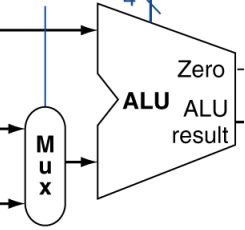
\includegraphics[scale=0.5]{alu_mux.png}    
\caption{MUX Before ALU}
\end{center}
\end{figure}

Figure 2 shows the first step that this program performs in instruction execute stage. Since the instruction decode stage generated control signals such as \texttt{ALUSrc} and \texttt{ALUOp}, the \texttt{MUX} needs to determine the input for ALU based upon those signals. As we all know, when \texttt{ALUSrc} is set 1, this means the ALU should take in immediate value as its second input. On the other hand, if the value was set as 0, the ALU is expecting for a value from register file which is \texttt{ReadData2}. 

Once the \texttt{MUX} has determined which value to send into ALU, it is now time for generating the ALU control signal. Since the stage when ALU control signal is generated was quite vague, in this program it assumes that this is done in execution stage. As mentioned in the textbook, unlike PLA for control signals, the logic gates for generating ALU control signal is quite accurate. 

\begin{figure}[h]
\begin{center}
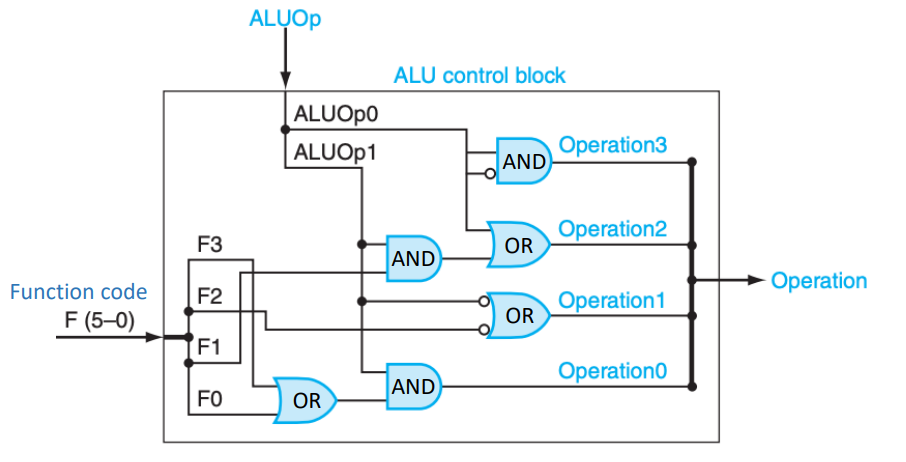
\includegraphics[scale=0.45]{alu_control_signal.png}    
\caption{Simple Combinational Logic Gate for ALU Control Signals}
\end{center}
\end{figure}

Just like the Figure 3, we need to implement a simple logic circuit using \texttt{C}. It is obvious fact that \texttt{C} supports direct access to bit modification, this can be done like following code snippet.
\\
\begin{center}
\begin{code}
\begin{minted}[frame=single,framesep=10pt]{c}
...
uint8_t operation;
uint8_t function_code= GET_FUNCT(cpu_instruction);

// Operation Code 0 is (F0 OR F3) AND ALUOp1.
operation = ((BIT_0(function_code) | BIT_3(function_code)) & alu_op_1) & 0x1;
// Operation Code 1 is ~F2 OR ~AluOp1.
operation = (((~BIT_2(function_code) | ~alu_op_1) & 0x1) << 1) | operation;
// Operation Code 2 is (F1 AND AluOp1) OR AluOp0.
operation = ((((BIT_1(function_code) & alu_op_1) | alu_op_0) & 0x1) << 2) 
            | operation;
// Operation Code 3 is (AluOp0 AND ~AluOp0) shall be 0.
operation = (((alu_op_0 & ~alu_op_0) & 0x1) << 3) | operation;
...
\end{minted}
\captionof{listing}{Code Snippet for Generating ALU Control Signals}
\end{code}
\end{center}
The full code for this snippet can be found under \texttt{generate_alu_control_signal} function implemented in \texttt{processor.c}. With the generated ALU control signal, it is now time to actually run ALU with the signals. With those signals, ALU is expected to behave like the following table.
\\
\begin{figure}[h]
\begin{center}
\begin{tabular}{|l|l|l|l|l|l|l}
    \hline
    \textbf{Opcode} & \textbf{ALUOp} & \textbf{Operation} & \textbf{Funct} & \textbf{ALU Function} & \textbf{ALU Control} \\
    \hline
        lw & 00 & Load Word & XXXXXX & Add & 0010 \\
        sw & 00 & Store Word & XXXXXX & Add & 0010 \\
        beq & 01 & Branch Equal & XXXXXX & Subtract & 0110 \\
        R-type & 10 & Add & 100000 & Add & 0010 \\
         & & Subtract & 100010 & Subtract & 0110 \\
         & & AND & 100100 & AND & 0000 \\
         & & OR & 100101 & OR & 0001 \\
         & & Set-on-Less-Than & 101010 & Set-on-Less-Than & 0111 \\
    \hline
\end{tabular}
\caption{Table of ALU Control Signals and ALU Behaviors}
\end{center}
\end{figure}
\\
However, if we just implement ALU following that table, our emulator will not perform as intended. This is due to some edge cases that fall short in that table. The following list are the instructions that are identified as some edge cases in the program:

\begin{itemize}
    \item \texttt{MULT}: The instruction will fall into ALU control of \texttt{0010} which is add. However, this needs to multiply the input values and store them inside \texttt{hi} and \texttt{lo}. 
    \item \texttt{BEQ}: The instruction will fall into ALU control of \texttt{0110} which is subtract. However, this also needs to check if the subtracted value is 0 to set \texttt{zero} value of ALU output for branch operations. 
    \item \texttt{BNE}: Just like \texttt{BEQ}, this also needs to check if the subtracted value is not 0 to set \texttt{zero} output for ALU in branch operations.
    \item \texttt{MFHI}: The instruction will fall into ALU control of \texttt{0110} which is subtract. However, this is expected to retrieve the \texttt{hi} value of \texttt{MULT}. Therefore this needs to set \texttt{ALUResult} as the \texttt{hi}.
    \item \texttt{MFLO}: Just like \texttt{MFHI}, the ALU should return \texttt{ALUResult} as \texttt{lo}. 
\end{itemize}

Please be advised that the list mentioned up above can differ from how actual MIPS architecture works. Also this might have potential errors and might not cover edge cases which resides outside of the program's expected instruction sets. With those exceptions, we can implement the ALU behavior as intended. The actual implementation of ALU resides as \texttt{alu} function under \texttt{processor.c}. The code is too long to be included into the snippet, therefore this will not be discussed in this document.

Once the ALU calculates \texttt{ALUResult} and \texttt{Zero}, it is now time for setting the \texttt{PC} value. The datapath for determining \texttt{PC} can be expressed as following figure.

\begin{figure}[h]
\begin{center}
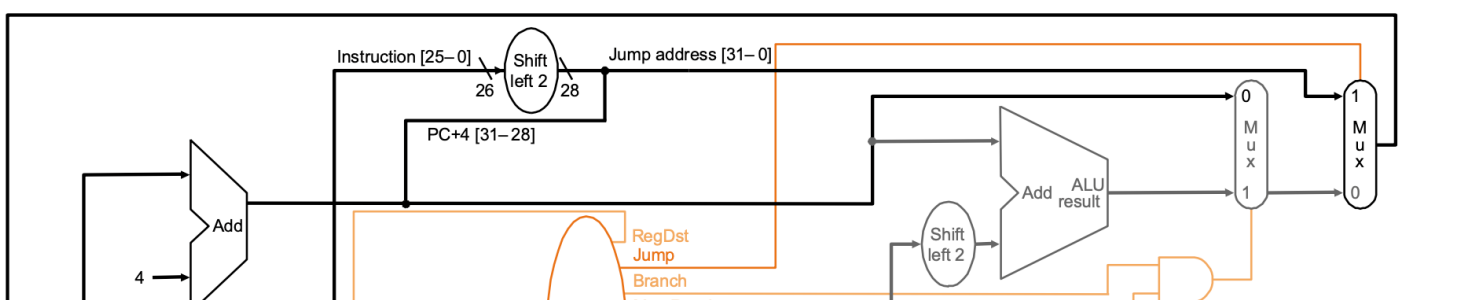
\includegraphics[scale=0.45]{determine_pc.png}    
\caption{Circuit for Determining PC}
\end{center}
\end{figure}

Using those datapaths mentioned in the Figure 5 can make our program determine which address to take. As mentioned in the instruction decode stage, we have already calculated \texttt{PC = PC + 4} before. Therefore, the only thing that is required is to determine the address for setting PC. This involves in two major signals: \texttt{Jump} and \texttt{Branch}. With those signals, we are able to determine the actual address that we can set \texttt{PC} as. 

For \texttt{Jump} signals, as we all know, converting 26 bit jump address from PC requires shifting left two times and then adding upper 4 bits of \texttt{PC}. This will make 26bit address into 32bit address which covers all the address of MIPS memory space. Then we let \texttt{MUX}es in the stage determine where to jump into. However, just like ALU, there are some exceptions that should be considered: \texttt{JAL} and \texttt{JR}.

\begin{itemize}
    \item \texttt{JR}: This instruction actually is R type instruction instead of J type instruction. Therefore, the control signal \texttt{Jump} should be set 1 for this instruction in the instruction decode stage. Also, the instruction is required to move \texttt{PC} into the value in \texttt{RS}. Since the \texttt{ALUResult} includes \texttt{RS}, this should directly set \texttt{ALUReuslt} instead of using the calculated jump address.
    \item \texttt{JAL}: Unlike other J type instructions, this instruction is expected to set \texttt{RA} as \texttt{PC} first and then set \texttt{PC} as calculated jump address.
\end{itemize} 
With those two extra considerations, the program implements jump related actions like following code snippet. The actual code implemention of this function can be found under \texttt{mips_execute} which resides in \texttt{processor.c}.
\\
\begin{center}
\begin{code}
\begin{minted}[frame=single,framesep=10pt]{c}
...
uint32_t jump_addr = GET_ADDR(cpu_instruction);
jump_addr = jump_addr << 2; 
jump_addr = jump_addr | GET_PC_UPPER(tmp_pc); 
if (signals.jump) {
    if (GET_FUNCT(cpu_instruction) == FUNCT_JR) {
        ctx->pc = ctx->alu_result;
    } else if (GET_OPCODE(cpu_instruction) == OPCODE_JAL) { 
        ctx->reg_map[RA] = ctx->pc;
        ctx->pc = jump_addr;
    }
} else {
    ctx->pc = tmp_pc;
}
...
\end{minted}
\captionof{listing}{Determining PC Value}
\end{code}
\end{center}
With the function that was implemented, the program is able to actually set \texttt{PC} addresses according to the input instructions. An example output of executing instruction \texttt{0x03e00008} which is \texttt{JR \$ra} is as it follows:
\\
\begin{center}
\begin{code}
\begin{minted}[frame=single,framesep=10pt]{c}
...
[DEBUG] OPCODE(0):
   - Signals: RegDst=1,AluSrc=0,MemToReg=0,RegWrite=0,MemRead=0,MemWrite=0,
              Branch=1,AluOp0=0,AluOp1=1,Jump=1
...
3) Execute - ALU Control (0x3)
   - ALU Result: 0xffffffff / Zero 0
   - Jump taken, PC = 0xffffffff
   - Update new PC: 0xffffffff
...
\end{minted}
\captionof{listing}{Example debug output for instruction \texttt{0x03e00008}}
\end{code}
\end{center}
As shown in the output, the program can generate signal \texttt{Jump} as 1. With the given signal, in the execute stage, the program can actually jump into \texttt{0xFFFFFFFF} which is the return address of the program. Since we have determined the jump address, it is now time for the next stage: memory read and write.
\pagebreak
\subsubsection{Memory Read and Write}
Compared to instruction decode and instruction execute, this stage is kind of easy and straight forward process. However, since this stage directly uses memory addresses to read and write data, this has the most room for errors like the infamous \textit{segfault}. Before actually accessing memory address, the program will check if the range of address is valid. Since our stack size is limited to \texttt{0x01000000}, the valid memory address will be \texttt{0x00000000} to \texttt{0x01000000}. 

Once the program checks the memory address, the program will now calculate offset based upon the memory address requested. This program stores memory using pure bytes. That means, the memory is implemented via \texttt{char *}. Therefore, calculating the offset will be performed like following code snippet.
\\
\begin{center}
\begin{code}
\begin{minted}[frame=single,framesep=10pt]{c}
...
char* offset = (char *)ctx->mem;
void* ret = NULL;
offset = offset + ctx->alu_result;
...
\end{minted}
\captionof{listing}{Code Snippet for Calculating Offset}
\end{code}
\end{center}
The program will calculate offset as the code snippet. The full code of this function can be found in \texttt{mips_load_store} in \texttt{processor.c}. Once the program has determined the offset for the address, it is time for actually reading and writing data from and to memory. 

For writing data from memory, the following code snippet is involved:
\\
\begin{center}
\begin{code}
\begin{minted}[frame=single,framesep=10pt]{c}
...
if (signals.mem_write) { 
    ret = memcpy(offset, &ctx->read_data_2, 4); 
    if (!ret) { // memcpy failed.
        return -1;
    }
}
...
\end{minted}
\captionof{listing}{Code Snippet for Reading Data from Memory}
\end{code}
\end{center}
As the code snippet insists, the program first checks for the signal \texttt{MemWrite} which was generated from instruction decode stage. If the signal was set 1, the program will write data into the designated offset using \texttt{memcpy} from \texttt{ReadData2}.  If the \texttt{memcpy} failed due to some reason, the program terminates execution in order to prevent from more errors. An example output for this code snippet using instruction \texttt{0xafc40028}, which is \texttt{SW \$a0 0x0028 \$fp}, is as it follows:
\pagebreak
\\
\begin{center}
\begin{code}
\begin{minted}[frame=single,framesep=10pt]{c}
...
[DEBUG] OPCODE(2b):
   - Signals: RegDst=0,AluSrc=1,MemToReg=0,RegWrite=0,MemRead=0,MemWrite=1,
              Branch=0,AluOp0=0,AluOp1=0,Jump=0
...
4) Memory Write - Address(0x00fffea0)
   - Successfully written 0x00000000 to Address 0x00fffea0
...
\end{minted}
\captionof{listing}{Example debug output for instruction \texttt{0xafc40028}}
\end{code}
\end{center}
As you can see, the program successfully stores data \texttt{0x00000000} into \texttt{0x00FFFEA0} which is the target address. Just like memory write, the program can read data from the memory using following code snippet. Again, the full code can be found under \texttt{mips_load_store} function under \texttt{processor.c}.
\\
\begin{center}
\begin{code}
\begin{minted}[frame=single,framesep=10pt]{c}
...
if (signals.mem_read) { 
    ret = memcpy(&ctx->mem_read_data, offset, 4); // Read data from memory.
    if (!ret) { // memcpy failed.
        return -1;
    }
}
...
\end{minted}
\captionof{listing}{Code Snippet for Writing Data into Memory}
\end{code}
\end{center}
The program will check for the signal \texttt{MemRead} which was generated from the instruction decode stage. Once the program finds out that the \texttt{MemRead} signal was set 1, the program will read data from the designated memory address using \texttt{memcpy}. Then the program will check if the reading data from memory was successful nor not to prevent any further errors if there was one. The read data will be stored to \texttt{mem_read_data} which will be forwarded to the next stage. An example output for this code snippet using \texttt{0x8fc20028}, which is \texttt{LW \$v0 0x0028 \$fp}, is as it follows.
\\
\begin{center}
\begin{code}
\begin{minted}[frame=single,framesep=10pt]{c}
...
[DEBUG] OPCODE(23):
   - Signals: RegDst=0,AluSrc=1,MemToReg=1,RegWrite=1,MemRead=1,MemWrite=0,
              Branch=0,AluOp0=0,AluOp1=0,Jump=0
...
4) Memory Read - Address(0x00fffea0)
   - Successfully Read 0x00000000 from Address 0x00fffea0
...
\end{minted}
\captionof{listing}{Example debug output for instruction \texttt{0x8fc20028}}
\end{code}
\end{center}
After this stage, the program will now continue with the last stage: register file write back.

\pagebreak
\subsubsection{Register File Write Back}
This stage is also one of the simple ones just like memory read and write stage. However, since this involves in storing data into register file, which was implemented as a \texttt{uint32_t} array, the program should be careful not to trigger \texttt{SEGSEV}. 

The program will first check the signal \texttt{MemToReg}. Once the signal was set as 1, the program will set \texttt{MUX} in a manner that the data coming from \texttt{ReadData} which was retrieved in the memory read stage can be directed into the register map. Otherwise, the \texttt{MUX} will direct the data from \texttt{ALUResult} into the register map. Then another \texttt{MUX} will set the target register according to \texttt{RegDst}. Once \texttt{RegDst} was set 1, the program will store data into register.\texttt{RD}, if this was set as 0, the program wills tore data to register \texttt{RT}. The code snippet that takes care of this part is as it follows. The full code can be found in function \texttt{mips_write_back} under \texttt{processor.c}.
\\
\begin{center}
\begin{code}
\begin{minted}[frame=single,framesep=10pt]{c}
...
uint32_t to_store = MUX(ctx->mem_read_data, ctx->alu_result, 
                        signals.mem_to_reg);
uint8_t write_register = MUX(GET_RD(cpu_instruction), GET_RT(cpu_instruction),
                         signals.reg_dst);
...
\end{minted}
\captionof{listing}{Code Snippet for MUX in Register Write}
\end{code}
\end{center}

Once the data source and register target was determined by two \texttt{MUX}es, the program will check for the signal \texttt{RegWrite}. If the signal was turned on, the program will store data into register file like following code snippet. Again, the full code is in \texttt{mips_write_back} under \texttt{processor.c}.
\\
\begin{center}
\begin{code}
\begin{minted}[frame=single,framesep=10pt]{c}
...
if (signals.reg_write) { // If this had RegWrite set 1, write to register file.
    if (write_register > REGISTER_COUNT || to_store < 0) { 
        return -1;
    } else { // If valid, store data.
        ctx->reg_map[write_register] = to_store;
        if (write_register != 0) SET_USED_REG(ctx->used_map, write_register);
    }
}
...
\end{minted}
\captionof{listing}{Code Snippet for Writing Data into Register File}
\end{code}
\end{center}
In this way, the program can actually store data into register file successfully. The example output using instruction \texttt{0x27bd0020}, which is \texttt{ADDIU \$sp \$sp 0x0020}, is as it follows.
\pagebreak
\\
\begin{center}
\begin{code}
\begin{minted}[frame=single,framesep=10pt]{c}
...
[DEBUG] OPCODE(9):
   - Signals: RegDst=0,AluSrc=1,MemToReg=0,RegWrite=1,MemRead=0,MemWrite=0,
              Branch=0,AluOp0=0,AluOp1=0,Jump=0
...
5) Register Write
   - Target Register: 29 / Value: 0x01000000
...
\end{minted}
\captionof{listing}{Example debug output for instruction \texttt{0x27bd0020}}
\end{code}
\end{center}
As the output indicates, the program can successfully store register data into the target register, in this case \texttt{\$sp} with value of \texttt{0x01000000}. 

\subsubsection{Limitations}
There was a trade-off between implementing MIPS architecture as much as possible and technical limitations due to lack of skills in \texttt{C} programming. Therefore, there were some limitations in this program. Those limitations are as it follows:
\begin{itemize}
    \item \textbf{Capturing Traps}: In MIPS architecture, there are some instructions which supports traps. \texttt{ADDU} and \texttt{ADDIU} are part of them. Since adding two register values in ALU might have an overflow, MIPS architecture gets us a trap so that we can actually recognize something went wrong. However, I have not implemented the trap and overflow detection in this program. Instead, the \texttt{ADDU} and \texttt{ADDIU} will be treated just like \texttt{ADD} and \texttt{ADDI} respectively. 
    \item \textbf{Unsupported Instructions}: In this program there are a handful set of instructions which are not implemented. Among those, the floating point operations are one of them. They are not required to be implemented by the homework therefore is not implemented.
    \item \textbf{No Memory Protection}: The program implements the whole memory using a big array of \texttt{char}s. The text region starts from \texttt{0x00000000} and the stack grows from \texttt{0x01000000} towards the \texttt{0x00000000}. In modern computers, stack overflowing into text region should not be possible. However, in this program it does not. For example, if you store data into \texttt{0x00000020}, the text region will change. Resulting in a possible instruction change. Also, if the stack grows too much and invades the text region, the program will lose instructions in text region. 
    \item \textbf{Counts \texttt{Nop}}: This is rather a policy not a limitation. However it seems like this is the right place to mention this subject. The instruction \texttt{0x00000000}, which is \texttt{Nop}, will counted as a R type instruction. Since the instruction will not do anything, this will just set the R type instruction counter by one and do nothing. This is to show that there is actually an instruction but not being executed.
    \item \textbf{Size Limitations}: The program utilizes \texttt{16MB} of memory by \texttt{malloc}. In modern systems, where \texttt{16MB} is not a big deal, however there might be errors with malloc for \texttt{16MB} for some environments. For example, if you run this program in a tight resource environment, such as containers with memory restriction via cgroups, VMs with memory limits, the program might be killed due to OOM.
\end{itemize}

\pagebreak
\section{User Guide \& Environments}
\subsection{Environment}
The environment that this program was checked running is as it follows:
\begin{itemize}
    \item \textbf{OS}: Ubuntu 22.04.01 LTS \textbf{Little Endian}
    \item \textbf{CPU}: Intel(R) Core(TM) i9-7940X CPU @ 3.10GHz
    \item \textbf{RAM}: 64GB
    \item \textbf{Compiler}: GCC 11.3.0, Make 4.3
    \item \textbf{C}: C99
\end{itemize}

Please be aware that with some environments, the program might not be able to execute. Also, with the code was zipped with version \texttt{Zip 3.0}. 

\subsection{User Guide}
\subsubsection{Unzipping}
Once you have downloaded the attached \texttt{.zip} file, you first need to unzip the file using following command.
\\
\begin{center}
\begin{code}
\begin{minted}[frame=single,framesep=10pt]{bash}
$ unzip FILE_NAME.zip
\end{minted}
\captionof{listing}{Unzip Command Example}
\end{code}
\end{center}
\\
Please change the \texttt{FILE\_NAME.zip} to the file that I have attached accordingly.

\subsubsection{Building}
Once you have unzipped the attached file, there will be a directory named \texttt{mipsim2}. Navigate to the directory \texttt{mipsim2} by using \texttt{cd}. \texttt{mipsim2} supports \texttt{make} with following recipes:
\begin{itemize}
    \item \texttt{debug}: For building debug version executable program with \texttt{--DDEBUG} option.
    \item \texttt{all}: For building executable program.
    \item \texttt{clean}: For cleaning up all \texttt{.o} files and generated executable program.
\end{itemize}

For example, if you were to build yourself a version for end-user case, use following command:
\\
\begin{center}
\begin{code}
\begin{minted}[frame=single,framesep=10pt]{bash}
$ make
gcc -O2 -Wall -std=gnu99 -o processor.o -c processor.c
gcc -O2 -Wall -std=gnu99 -o context.o -c context.c
gcc -O2 -Wall -std=gnu99 -o io.o -c io.c
gcc -O2 -Wall -std=gnu99 -o main.o -c main.c
gcc -o mipsim processor.o context.o io.o main.o
\end{minted}
\captionof{listing}{Example Build Output}
\end{code}
\end{center}
\\
This will generate object files ending with \texttt{.o} as well as an executable file named \texttt{mipsim}. To clean up your workspace, use \texttt{clean} recipe for removing all generated files.

\subsubsection{User Guide}
\texttt{mipsim} offers simple command line interfaces. You can use following command to get a glimpse of each options:
\\
\begin{center}
\begin{code}
\begin{minted}[frame=single,framesep=10pt]{bash}
$ ./mipsim  --help
...
A Bit more complex Single Cycle MIPS Simulator
                            32190984 Isu Kim
Usage: mipsim [options]
Options
  -h, --help           Print this help message and exit
  -i, --input          Specify an input file to execute
\end{minted}
\captionof{listing}{Example Help Output}
\end{code}
\end{center}

The options are:
\begin{itemize}
    \item \texttt{help}: For printing out the help message.
    \item \texttt{input}: For specifying an input file. This is required parameter.
\end{itemize}

For example, an example execution command will be:
\\
\begin{center}
\begin{code}
\begin{minted}[frame=single,framesep=10pt]{bash}
$ ./mipsim  -i input.txt
...
A Bit more complex Single Cycle MIPS Simulator
                            32190984 Isu Kim
[INFO] Input File: ./inputs/prof_input1/input.bin
[INFO] Starting simulator
\end{minted}
\captionof{listing}{Example Command Line Interface Output}
\end{code}
\end{center}

This will execute an file named \texttt{./inputs/prof_input1/input.b} and print out the results.

\warningbox{As defined in \texttt{common.h}, the maximum memory size of this program is the total stack size which is 16MB. Also the file name's max string length is 1024. Any files which are bigger than 16MB or having a longer file name than 1024 bytes might cause failure of the program.} 

\pagebreak
\subsubsection{Available Instructions}
\\
The program supports instructions from MIPS green sheet. However, there are some instructions that are fully supported, semi-supported and not supported. The following table indicates the instructions that are \textbf{fully} supported.

\begin{figure}[h]
\begin{center}
\begin{tabular}{|l|l|l|l|l|}
    \hline
        \textbf{Name} & \textbf{opcode} & \textbf{Function Code} & \textbf{Comments}\\
    \hline
        add & 0x00 & 0x20 & N/A\\
        addi & 0x08 & N/A & N/A\\
        and & 0x00 & 0x24 & N/A\\
        andi & 0x0c & N/A & N/A\\
        beq & 0x04 & N/A & N/A\\
        bne & 0x05 & N/A & N/A\\
        j & 0x02 & N/A & Theoretically implemented\\
        jal & 0x03 & N/A & N/A\\
        jr & 0x00 & 0x08 & N/A\\
        lw & 0x23 & N/A & N/A\\
        or & 0x00 & 0x27 & N/A\\
        ori & 0x0d & N/A & Theoretically implemented\\
        slt & 0x00 & 0x2a & N/A\\
        slti & 0x0a & N/A & N/A\\
        sw & 0x2b & N/A & N/A\\
        sub & 0x00 & 0x22 & N/A\\
        mult & 0x00 & 0x18 & N/A\\
        mfhi & 0x00 & 0x10 & N/A\\
        mflo & 0x00 & 0x12 & N/A\\
    \hline
\end{tabular}
\caption{Table of Fully Supported Instructions}
\end{center}
\end{figure}
\\
The following table shows list of instructions that are not implemented perfect. 

\begin{figure}[h]
\begin{center}
\begin{tabular}{|l|l|l|l|l|}
    \hline
        \textbf{Name} & \textbf{opcode} & \textbf{Function Code} & \textbf{Comments}\\
    \hline
        addu & 0x00 & 0x21 & Trap not detected, will behave like \texttt{add}\\
        addiu & 0x09 & N/A & Trap not detected, will behave like \texttt{addi}\\
        sltiu & 0x0b & N/A & Trap not detected, will behave like \texttt{slti}\\
        sltu & 0x00 & 0x2b & Trap not detected, will behave like \texttt{slt}\\
        subu & 0x00 & 0x22 & Trap not detected, will behave like \texttt{sub}\\
    \hline
\end{tabular}
\caption{Table of Semi-Supported Instructions}
\end{center}
\end{figure}
\\
Any instructions not mentioned here are not implemented. With those implemented instructions, this program was verified to run both the input files that Professor Nam gave us: input1 and input2. 
\warningbox{Using any unsupported instructions will not only result in unexpected behavior but also might have potential for crashing the program.} 
\pagebreak

\subsubsection{Demonstrations}
In order to verify if \texttt{mipsim} works properly or not, the list below is the codes that were tested working on \texttt{mipsim}. Also codes are included in the attachments, so you can try them yourself.

\begin{itemize}
    \item \texttt{inputs/compile.sh}: A simple shell file that compiles a \textt{.c} into \texttt{.bin} and \texttt{.s}. But this requires editing addresses using \texttt{hexedit -l 4 filename}.
    \item \texttt{inputs/new_factorial/factorial.bin}: Simple binary uses recursion to solve $5!$. 
    \item \texttt{inputs/new_fibonacci/fibonacci.bin}: Simple binary uses recursion to solve 15th number of fibonacci.
    \item \texttt{inputs/prof_input1/input.bin}: The first input that Professor offered us.
    \item \texttt{inputs/prof_input2/input.bin}: The second input that Professor offered us.
\end{itemize}

A screenshot of executing \texttt{inputs/prof_input1/input.bin} is as it follows:

\begin{figure}[h]
\begin{center}
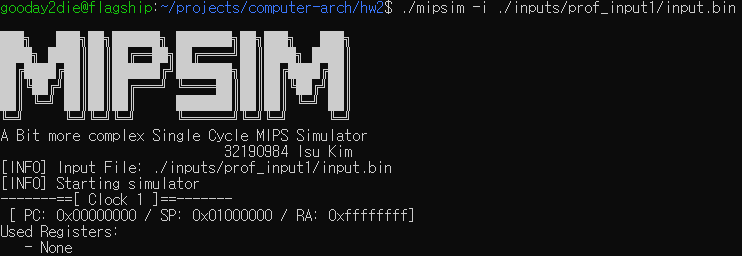
\includegraphics[scale=0.8]{screenshot_1.png}    
\caption{Screenshot - Input Executing Input 1}
\end{center}
\end{figure}

\begin{figure}[h]
\begin{center}
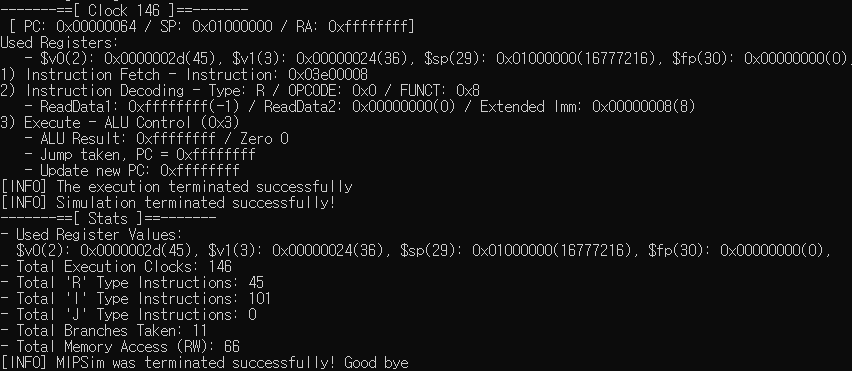
\includegraphics[scale=0.7]{screenshot_2.png}    
\caption{Screenshot - Final Result Executing Input 1}
\end{center}
\end{figure}
\warningbox{This program actually executes instruction \texttt{0x00000000}, which is \texttt{Nop}. Since the opcode for \texttt{Nop} is \texttt{0x00}, the program will count this as a R type instruction executed.} 

\pagebreak
The program prints out information of current state in every clock cycle. In each clock cycles, the program prints out information in a format like below:
\begin{figure}[h]
\begin{center}
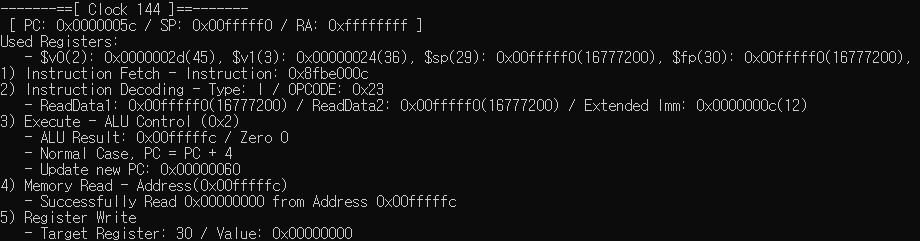
\includegraphics[scale=0.7]{screenshot_3.png}    
\caption{Screenshot - Example Output for Single Cycle}
\end{center}
\end{figure}

In the screenshot, which is the 144th clock of the \texttt{/inputs/prof_input1/input.bin}, the program executes instruction \texttt{0x8fbe000c}. The instruction can be translated to \texttt{LW \$fp 0x000C \$sp}. The program prints out each stages of the program. With the output screen, we can identify following information.
\begin{enumerate}
    \item \textbf{\texttt{PC}}: The \texttt{PC} address is \texttt{0x0000005c}.
    \item \textbf{Instruction Fetch}: The program fetched instruction \texttt{0x8fbe000c}. 
    \item \textbf{Instruction Decode}: The program detected the instruction as I type instruction with opcode \texttt{0x23}. Also the \texttt{ReadData1} and \texttt{ReadData2} was retrieved from regsiter as respective values. On the otherhand, the immediate was extended to 32bits with keeping the value \texttt{12}.
    \item \textbf{Execute}: The ALU received ALU control signal of \texttt{0x2}, which is \texttt{0b0010}. That will perform add. Also, the result was calculated as \texttt{0x00fffffc} with \texttt{zero} set as 0. So this was a normal case, meaning that the program does not have to do jump or branch instruction. This will just perform \texttt{PC = PC + 4}.
    \item \textbf{Memory Read}: The program read data from \texttt{0x00fffffc} which was the address calculated from the ALU. The read data was \texttt{0x00000000}.
    \item \textbf{Register Write}: After the read data was retrieved, the program is writing data to register \texttt{30} with value of \texttt{0x00000000}.
\end{enumerate}
If you would like to see a better in depth action and what actually is going on inside the ALU, compile the program with debug option. 
\\
\begin{center}
\begin{code}
\begin{minted}[frame=single,framesep=10pt]{bash}
$ make debug
gcc -O2 -Wall -std=gnu99 -DDEBUG -o context.o -c context.c
gcc -O2 -Wall -std=gnu99 -DDEBUG -o io.o -c io.c
gcc -O2 -Wall -std=gnu99 -DDEBUG -o main.o -c main.c
gcc -o mipsim processor.o context.o io.o main.o
\end{minted}
\captionof{listing}{Compiling the Program with Debug Option}
\end{code}
\end{center}
With the debug option, we can now have better insights on how everything is taking place. An example screenshot for a single cycle is as it follows:

\begin{figure}[h]
\begin{center}
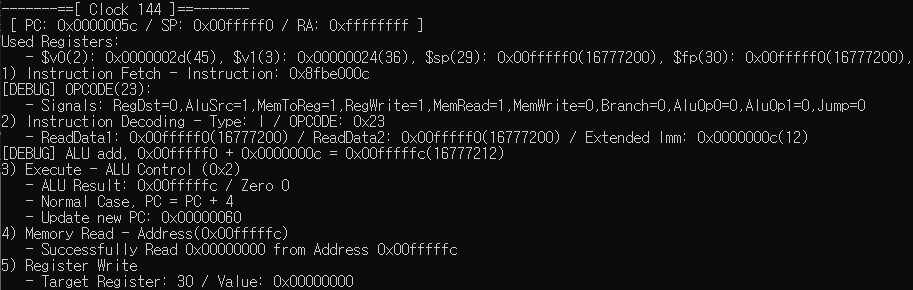
\includegraphics[scale=0.7]{screenshot_4.png}    
\caption{Screenshot - Debug Output for Single Cycle}
\end{center}
\end{figure}
\\
The debug screen shows more information on the details, such as signals generated in instruction decode stage and actual action taken in ALU. For example in instruction decode stage, the signals generated was like the table below:

\begin{figure}[h]
\begin{center}
\begin{tabular}{|l|l|l|l|l|l|l|l|l|l|}
    \hline
    \textbf{RegDst} & \textbf{AluSrc} & \textbf{MemToReg} & \textbf{RegWrite} & \textbf{MemRead} \\
    \hline
    0 & 1 & 1 & 1 & 1 \\
    \hline
    \textbf{MemWrite} & \textbf{Branch} & \textbf{AluOp0} & \textbf{AluOp1} & \textbf{Jump} \\
    \hline
    0 & 0 & 0 & 0 & 0 \\
    \hline
\end{tabular}
\caption{Generated Control Signals}
\end{center}
\end{figure}
Also with the given signals, ALU performs add with \texttt{0x00fffff0} and \texttt{0x0000000c}. So with the debug mode turned on, you can see more information inside the code.

From now on, we are going to take some demonstration codes included in \texttt{inputs} directory and check if they actually work in our program.

\warningbox{If you are trying to write a new code and insert it to verify the code, please check your inputs. Due to the binary that was generated by \texttt{boanlab\/mips-ubuntu}, sometimes the function definition sequence matters. Make sure that your \texttt{int main()} resides on top of your code. Meaning that no other function \textbf{declaration} should not be held before \texttt{int main()}. If not, \texttt{main} function will not take the address of \texttt{0x00000000} which will result in not executing the main function.}

\pagebreak
\subsection{Inputs}
\subsubsection{\texttt{inputs/prof_input1/input.bin}}
The source code for for the binary input file is as it follows:
\\
\begin{center}
\begin{code}
\begin{minted}[frame=single,framesep=10pt]{bash}
int main() {
        int sum = 0;

        for (int i=0; i<10; i++)
                sum += i;

        return sum;
}
\end{minted}
\captionof{listing}{Input 1 - \texttt{inputs/prof_input1/input.c}}
\end{code}
\end{center}

Since the screenshot is quite difficult to see, I will be copying the result from the file into here fore better readability. The output execution result is as it follows: 
\\
\begin{center}
\begin{code}
\begin{minted}[frame=single,framesep=10pt]{bash}
...
[INFO] The execution terminated successfully
[INFO] Simulation terminated successfully!
-------==[ Stats ]==-------
- Used Register Values:
  $v0(2): 0x0000002d(45), $v1(3): 0x00000024(36) ...
- Total Execution Clocks: 146
- Total 'R' Type Instructions: 45
- Total 'I' Type Instructions: 101
- Total 'J' Type Instructions: 0
- Total Branches Taken: 11
- Total Memory Access (RW): 66
[INFO] MIPSim was terminated successfully! Good bye
\end{minted}
\captionof{listing}{Output 1 - \texttt{inputs/prof_input/input.bin}}
\end{code}
\end{center}
The program had job adding all values from 0 to 9. Therefore the result 45 stored in \texttt{\$v0} is correct.
\pagebreak

\subsubsection{\texttt{inputs/prof_input2/input.bin}}
The source code for for the binary input file is as it follows:
\\
\begin{center}
\begin{code}
\begin{minted}[frame=single,framesep=10pt]{bash}
int foo(int index);

int main() {
    int index = 4;
    return foo(index);
}

int foo(int index) {
    if (index == 1)
        return 1;
    else
        return index + foo(index-1);
}
\end{minted}
\captionof{listing}{Input 2 - \texttt{inputs/prof_input2/input.c}}
\end{code}
\end{center}

Since the screenshot is quite difficult to see, I will be copying the result from the file into here fore better readability. The output execution result is as it follows: 
\\
\begin{center}
\begin{code}
\begin{minted}[frame=single,framesep=10pt]{bash}
...
[INFO] The execution terminated successfully
[INFO] Simulation terminated successfully!
-------==[ Stats ]==-------
- Used Register Values:
  $v0(2): 0x0000000a(10), $v1(3): 0x00000006(6), $a0(4): 0x00000001(1), ...
- Total Execution Clocks: 99
- Total 'R' Type Instructions: 35
- Total 'I' Type Instructions: 60
- Total 'J' Type Instructions: 4
- Total Branches Taken: 4
- Total Memory Access (RW): 36
[INFO] MIPSim was terminated successfully! Good bye
\end{minted}
\captionof{listing}{Output 2 - \texttt{inputs/prof_input/input.bin}}
\end{code}
\end{center}
The program had job adding all values from 1 to 4. Therefore the result 10 stored in \texttt{\$v0} is correct.
\pagebreak

\subsubsection{\texttt{inputs/new_fibonacci/fibonacci.bin}}
The source code for for the binary input file is as it follows:
\\
\begin{center}
\begin{code}
\begin{minted}[frame=single,framesep=10pt]{bash}
int fibonacci(int n);

int main(void) {
    return fibonacci(15);
}

int fibonacci(int n) {
    if (n <= 1) {
        return n;
    }
    return fibonacci(n - 1) + fibonacci(n - 2);
}
\end{minted}
\captionof{listing}{Input 3 - \texttt{inputs/new_fibonacci/fibonacci.c}}
\end{code}
\end{center}

Since the screenshot is quite difficult to see, I will be copying the result from the file into here fore better readability. The output execution result is as it follows: 
\\
\begin{center}
\begin{code}
\begin{minted}[frame=single,framesep=10pt]{bash}
...
[INFO] The execution terminated successfully
[INFO] Simulation terminated successfully!
-------==[ Stats ]==-------
- Used Register Values:
  $v0(2): 0x00000262(610), $a0(4): 0x00000001(1), $s0(16): 0x00000000(0), ...
- Total Execution Clocks: 48345
- Total 'R' Type Instructions: 16771
- Total 'I' Type Instructions: 29601
- Total 'J' Type Instructions: 1973
- Total Branches Taken: 1973
- Total Memory Access (RW): 18747
[INFO] MIPSim was terminated successfully! Good bye
\end{minted}
\captionof{listing}{Output 3 - \texttt{inputs/prof_input/input.bin}}
\end{code}
\end{center}
The program had job finding the $15^{th}$ value of Fibonacci sequence.

\[
\text{{fib}}(15) = \frac{{\left(\frac{{1 + \sqrt{5}}}{2}\right)^{15} - \left(\frac{{1 - \sqrt{5}}}{2}\right)^{15}}}{{\sqrt{5}}} = 610
\]
As the equation gets us, the value of $15^{th}$ value of Fibonacci sequence is 610. Therefore the result 610 stored after 48345 clock cycles in \texttt{\$v0} is indeed correct.
\pagebreak

\subsubsection{\texttt{inputs/new_factorial/factorial.bin}}
The source code for for the binary input file is as it follows:
\\
\begin{center}
\begin{code}
\begin{minted}[frame=single,framesep=10pt]{bash}
int factorial(int n);

int main() {
    return factorial(5);
}

int factorial(int n) {
    if (n == 0 || n == 1) {
        return 1;
    } else {
        return n * factorial(n - 1);
    }
}
\end{minted}
\captionof{listing}{Input 3 - \texttt{inputs/new_factorial/factorial.c}}
\end{code}
\end{center}

Since the screenshot is quite difficult to see, I will be copying the result from the file into here fore better readability. The output execution result is as it follows: 
\\
\begin{center}
\begin{code}
\begin{minted}[frame=single,framesep=10pt]{bash}
...
[INFO] The execution terminated successfully
[INFO] Simulation terminated successfully!
-------==[ Stats ]==-------
- Used Register Values:
  $v0(2): 0x00000078(120), $v1(3): 0x00000018(24), $a0(4): 0x00000001(1), ...
- Total Execution Clocks: 144
- Total 'R' Type Instructions: 58
- Total 'I' Type Instructions: 81
- Total 'J' Type Instructions: 5
- Total Branches Taken: 5
- Total Memory Access (RW): 47
[INFO] MIPSim was terminated successfully! Good bye
\end{minted}
\captionof{listing}{Output 3 - \texttt{inputs/prof_input/input.bin}}
\end{code}
\end{center}
The program had job finding the value of $5!$. 

\[
5! = 5 \times 4 \times 3 \times 2 \times 1 = 120
\]

As the equation gets us, the value of $5!$ is 120. Therefore the result 120 stored in \texttt{\$v0} is indeed correct.
\pagebreak



\pagebreak
\section{Conclusion}

Implementing the single cycle MIPS emulator was an incredibly enjoyable project. I found it fascinating how the program could actually run simply by connecting the datapaths and control signals. Initially, I had doubts about whether just connecting those wires would work or not. However, this project provided me with a great opportunity to review what we learned in class about the single cycle CPU.

By working on this homework assignment, I have gained a better understanding of the single cycle architecture. This understanding will undoubtedly give me an advantage when learning about multicycle and pipelining in our next homework assignment.

Overall, I found the project to be both enriching and enlightening. It allowed me to apply the knowledge gained in class and see firsthand how the various components of a CPU come together to execute instructions. I'm grateful for the experience as it has deepened my understanding of computer architecture and motivated me to explore further in this field.

Implementing the single cycle MIPS emulator in C was a rewarding experience. It involved working at both the byte and bit level, which is especially easy to achieve in C. However, despite its rewarding nature, I encountered a few difficulties along the way. Here is a list of the challenges I faced throughout the project:

\begin{itemize}
    \item \textbf{Handling branch and jump instructions}: Branch and jump instructions introduced additional complexity to the project. Determining the correct target addresses and modifying the \texttt{PC} accordingly required careful handling and consideration of the instruction formats.
    \item \textbf{Managing memory}: Implementing memory access was challenging, especially when dealing with load and store instructions. Properly handling byte and word addresses and ensuring correct data retrieval and storage proved to be a tricky task. Otherwise, this have made a bunch of segfaults (which will have us a fun time debugging).
    \item \textbf{Handling exceptions}: Since implementing the MIPS architecture 100\% was quite impossible. Therefore there were quite gap between the actual implementation and the real architecture. In order to fill in the gap, some exception handling was required. 
\end{itemize}
Besides those difficulties, there were some lessons that I have learned throughout the journey of implementing MIPS emulator. 

\begin{itemize}
    \item \textbf{ChatGPT is stupid}: Honestly speaking, I have used ChatGPT for my documents. While ChatGPT has been helpful in assisting me with writing my document and organizing tables in LaTeX, it has some limitations when it comes to knowledge of the MIPS architecture. Also, it gave me some wrong macros in C, which eventually slowed down my process of developing this project a lot. Therefore, a lesson learnt, do not blind-fully trust on ChatGPT.
    \item \textbf{Research before designing}: I have wasted lot of time in implementing the control signal generator. At first, I have refereed to the PLA implementation and implemented that digital logic circuit using C. However, it turned out to be the PLA which had me stalled in this project for a long time. The PLA was not a correct version and it had some exceptions such as \texttt{ADDIU}. Therefore, researching more before i actually design the project will be one of the considerations in the next project. 
\end{itemize}

\end{document}
